% Prof. Dr. Ausberto S. Castro Vera
% UENF - CCT - LCMAT - Curso de Ci\^{e}ncia da Computa\c{c}\~{a}o
% Campos, RJ,  2015
% Disciplina: An\'{a}lise e Projeto de Sistemas
% Aluno:



\chapter{Conclus\~{o}es}


O trabalho trouxe grandes desafios, já que é uma grande documentação. Mas também me fez adquirir muito conhecimento a respeito
de Análise e Projeto de Sistemas.


Foi desenvolvido um sitema acadêmico, com toda sua forma de análise. 
 \begin{itemize}
  \item Planejamento
  \item Análise
  \item Projeto
 \end{itemize}


Poderia ser algo mais completo, pois a documentação é criada para aspecto só de trabalho, mas seria mais interessante se fosse
mais integrado com as matérias. Fazer toda a documentação e depois desenvolver o software, pois assim teriamos todo conhecimento
completo das etapas da criação do software.



   \begin{figure}[H]
    \begin{center}
        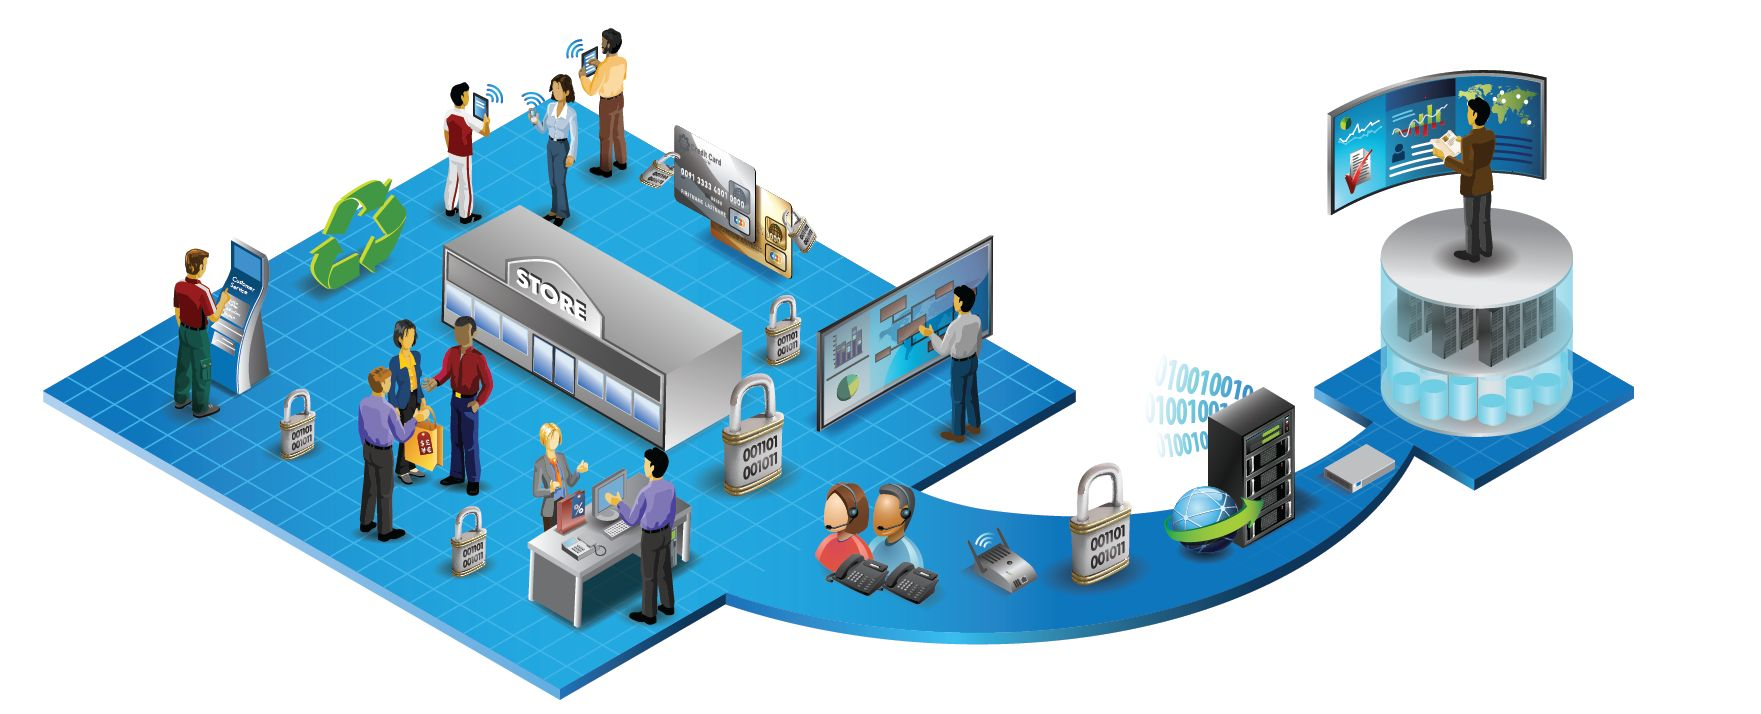
\includegraphics[width=12cm]{MeuSistema.jpg}
        \caption{Meu Sistema a ser desenvolvido} \label{sistema}
    \end{center}
   \end{figure} 